% -*- root: Dissertation.tex -*-
\documentclass[Dissertation.tex]{subfiles}
\begin{document}
\graphicspath{{../Figures/}}
\chapter{Scaling Issues}
\label{sec:Scaling}

\section{Global Solvers}
The one challenge which we most significantly underestimated before undertaking this work 
was how our solver would scale on these space-time problems.
Preliminary 1D results (2D in space-time), were computable with standard direct solvers,
but as we moved to 2D (3D in space-time), direct solvers proved to be a major bottleneck
to larger solves, not least of which because they tend to take up more memory than iterative solvers.
Fortunately, my collaborator Nathan Roberts has been implementing 
flexible multigrid strategies within Camellia.
Unfortunately, multigrid is well known to perform poorly on convection-dominated diffusion problems.
In fact, we can easily construct a case for convection-diffusion with $\epsilon=10^{-2}$ on a $64\times64$
mesh solved with Camellia's default multigrid strategy outlined below that
% mesh where a combination of conjugate gradient, v-cycle multigrid 
exhibits the convergence history in Figure~\ref{fig:ConfusionResidual} for the iterative solve.
% fails to converge to a tolerance of $10^{-10}$ within 2000 iterations.
\begin{figure}[!ht]
\centering
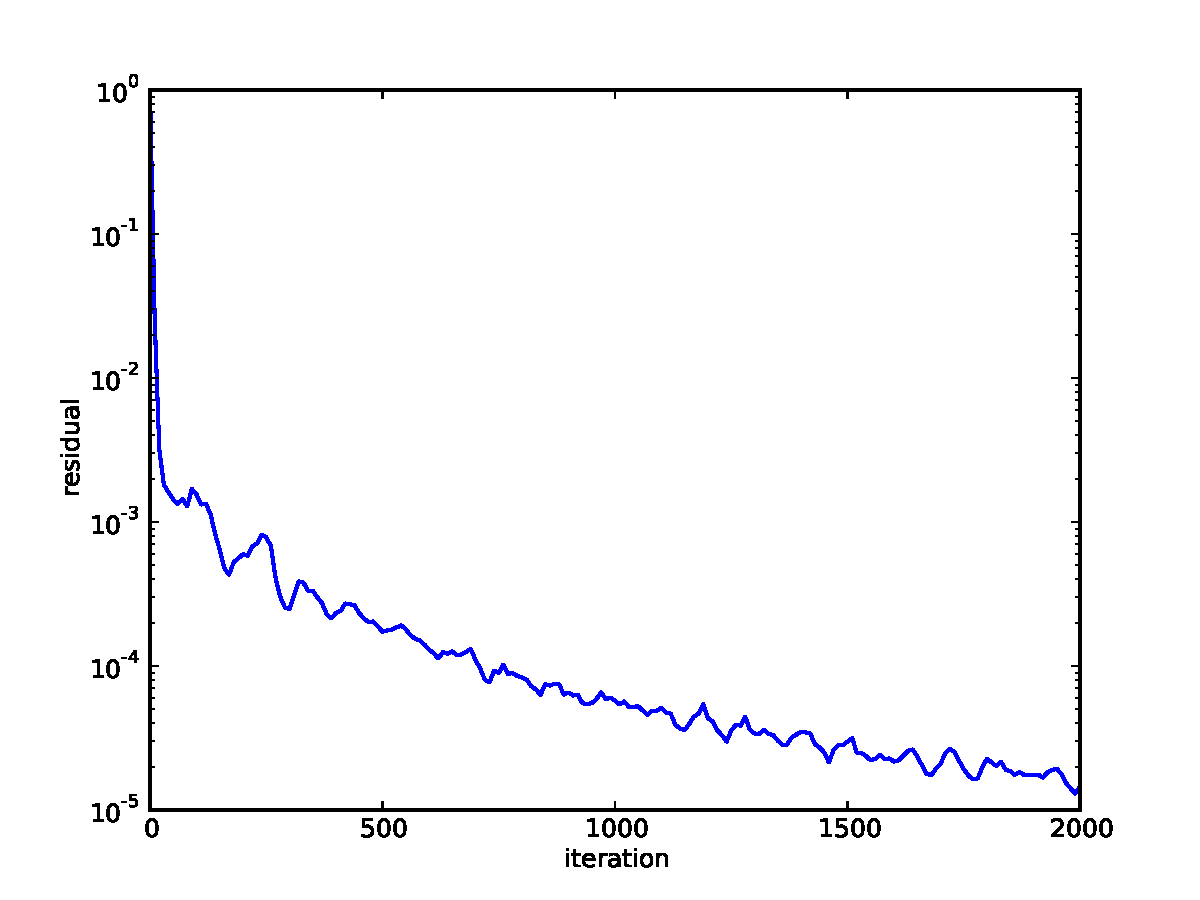
\includegraphics[width=\textwidth]{Dissertation/Scaling/ConfusionResidual.pdf}
\caption{Residual convergence for a simple convection-diffusion problem}
\label{fig:ConfusionResidual}
\end{figure}

The details of this simulation aren't important, the point is that it is fairly trivial to contrive a 
test problem where multigrid performs very poorly for convection-diffusion.
% In our experience, we've noticed that this tends to be somewhat mitigated on adaptive meshes rather rather than the uniform one used for this example.
This behavior appears to be especially bad on uniform meshes and seems to be somewhat mitigated on adaptive meshes.
Ideally we would like to implement a line smoother which is known to improve performance 
on convection-dominated diffusion problems, but that is outside the scope of this thesis.

\subsection{Overview of Multigrid in Camellia}
Conjugate gradient is a natural choice for iteratively solving DPG problems because they are always symmetric
(Hermitian) positive definite.
However a good preconditioner is necessary for efficiency.
My collaborator, Nathan Roberts at Argonne National Lab, implemented a geometric multigrid preconditioner
that has allowed us to solve larger problems than we could with direct solvers.
I've served as more of a user and tester of the multigrid strategies than as a developer, so
I'll only briefly describe an overview of the settings we settled on 
that were used in the simulations in this thesis.

After exploring the various options of additive or multiplicative two-cycle, V-cycle, W-cycle, or full multigrid,
we settled on a multiplicative V-cycle strategy.
We've chosen to employ an overlapping additive Schwarz smoother.
In constructing the mesh hierarchy for the multigrid, going from a high order fine mesh, we first start
with $p$-coarsening followed by $h$-coarsening.
More details on multigrid within Camellia will appear in an upcoming technical report by Nathan Roberts.

\subsection{Scaling on Test Problems}
% Support for space-time within Camellia is still fairly experimental and multigrid has 
Both space-time and multigrid are fairly recent, experimental features within Camellia
and the combination of the two has not scaled as well as we initially expected. 
In the following tables we illustrate the ballooning cost of these space-time solves 
for 2D incompressible Navier-Stokes.
A 2D space-time solver was implemented for compressible Navier-Stokes as well, but the 
scaling issues illustrated here for incompressible Navier-Stokes were significantly worse
in the presence of shocks. 
Despite significant effort, we were not able to obtain publishable results for any 2D shock problems.

\subsubsection{Incompressible Flow Over a Cylinder}
\label{sec:incompressibleCylinder}
Table~\ref{tab:cylinder} refers to a space-time solve of transient flow over a flat plate. 
Listed times are in seconds.
The domain is $[-3,9]\times[-4.5,4.5]$ with a 0.5 radius cylinder in at the origin and a final time of 4.
The Reynolds number is 100, the flow is initialized to the solution of potential flow over a cylinder.
Velocity conditions are applied to the inflow, zero slip to the cylinder, and zero traction to every other boundary.
The initial mesh has 80 space-time elements and with quadratic trial functions has 31304 DOFs 
and looks like Figure~\ref{fig:CylinderMesh0}.
After 4 adaptive refinements, the problem is up to 11742 elements, 4144674 DOFs, 
and looks like Figure~\ref{fig:CylinderMesh4}.
This problem was excluded from the main set of incompressible results in Chapter~\ref{sec:incompressible}
because we don't achieve nearly enough resolution to observe any interesting flow features.

\begin{figure}[!ht]
\centering
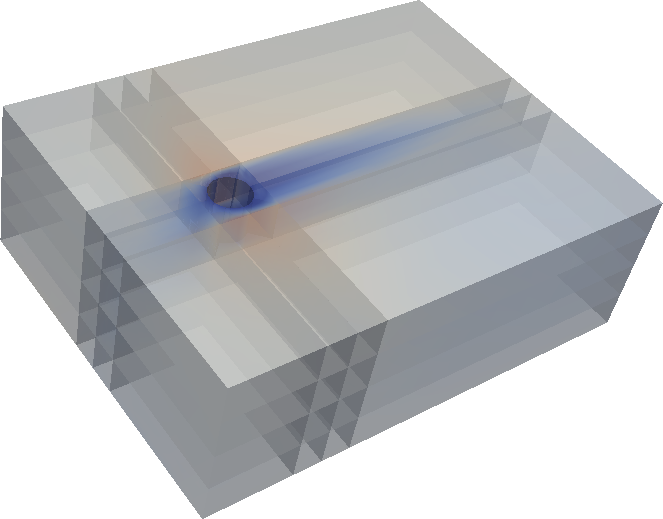
\includegraphics[width=\textwidth]{Dissertation/Cylinder/Mesh_uMag0.png}
\caption{Initial mesh for cylinder problem colored by velocity magnitude}
\label{fig:CylinderMesh0}
\end{figure}

\begin{figure}[!ht]
\centering
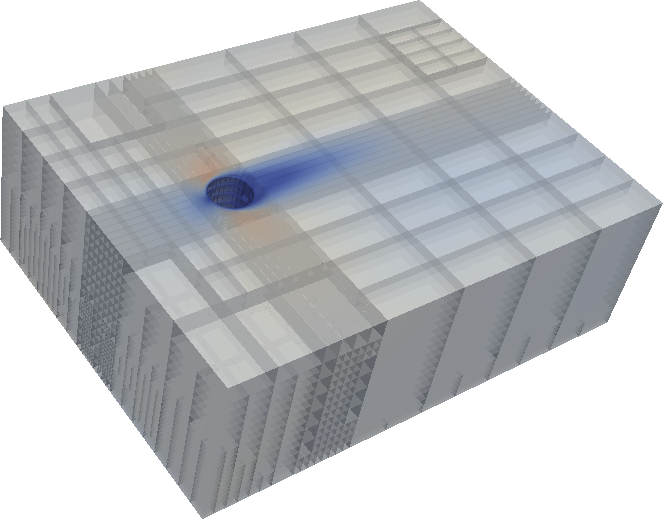
\includegraphics[width=\textwidth]{Dissertation/Cylinder/Mesh_uMag4.png}
\caption{Fourth adaptive mesh for cylinder problem colored by velocity magnitude}
\label{fig:CylinderMesh4}
\end{figure}

The cost per solve increases dramatically with every adaptive refinement step.
We compare three runs from done on the Lonestar system at the Texas Advanced Computing Center.
In the first, we use 1 node with 24 processors and then compare this to 4 nodes with 96 processors and
32 nodes with 768 total processors.
Strong scaling results are computed relative to the previous solve 
with ideal values being $4\times$ and $8\times$ for the 4 node and 32 node runs, respectively.
It is clear that increasing the number of processors does accelerate the solve, but we are not
very close to the ideal speedup.
We hypothesize that load balancing on this problem is sub-optimal as not ever processor has
to deal with curvilinear element computations around the cylinder.
With 768 processors, it takes more than 2 hours to complete 10 Newton iterations 
on the fourth refinement step with just over 4 million DOFs.
We estimate it would take about 6 refinement steps before we start resolving the viscous flow features.

\begin{table}[!ht]
\centering
\caption{Solve time for transient flow over a cylinder}
\label{tab:cylinder}
\begin{tabular}{|crr|r|rc|rc|}
\hline
& & & 1 Node & \multicolumn{2}{|c|}{4 Nodes} & \multicolumn{2}{|c|}{32 Nodes} \\
Ref& Elems & DOFs & Time    & Time & Scaling vs 1     & Time & Scaling vs 4      \\
\hline
0 & 80            & 31304      & 1772   & 453   & 3.91 & 451  & 1.01 \\
1 & 605           & 225908     & 8190   & 3574  & 2.29 & 717  & 4.98 \\
2 & 3013          & 1081598    & 32008  & 12076 & 2.65 & 2648 & 4.56 \\
3 & 9726          & 3429384    &          & 28744 &      & 6319 & 4.54 \\
4 & 11742         & 4144674    &          &         &      & 8510 &      \\
\hline
\end{tabular}
\end{table}

\subsubsection{Taylor-Green Vortex}
We also consider the Taylor-Green vortex problem described in Chapter~\ref{sec:incompressible}.
The timings for the case of $Re=1000$ and $p=2$ are shown in Table~\ref{tab:taylor}.
We see better scaling for this problem as there are not any curvilinear elements to deal with
but the time to solve still blows up considerable with every refinement step.

\begin{table}[!ht]
\centering
\caption{Solve time for the Taylor-Green vortex}
\label{tab:taylor}
\begin{tabular}{|crr|r|rc|}
\hline
& & & 1 Node & \multicolumn{2}{|c|}{4 Nodes} \\
Ref& Elems & DOFs & Time    & Time & Scaling vs 1 \\
\hline
0 & 60            & 21302      & 331.0    & 140.6   & 2.35 \\
1 & 312           & 108410     & 945.2    & 290.6   & 3.25 \\
2 & 2020          & 691834     & 4880.2   & 1363.5  & 3.58 \\
3 & 9244          & 3043024    &          & 6171.6  & \\
\hline
\end{tabular}
\end{table}

\section{The Question of Space-Time Slabs}
Here we briefly explore the benefits of splitting a computation into space-time slabs under the following assumptions.
\begin{enumerate}
\item The maximum required spatial resolution is much finer than the required temporal resolution.
\item Regions requiring high spatial resolution are concentrated in relatively compact parts of the domain.
\item Only isotropic refinements are permitted.
\item The number of time slabs is a power of 2.
\end{enumerate}
The first and second conditions are representative of the boundary layer and 
shock problems considered in this thesis.
The third condition is necessary as Camellia does not currently support anisotropic refinements in space-time.

Our test case is a steady boundary layer problem with exact solution
\[
u=1-e^\frac{x}{\epsilon}
\]
solved on a space-time domain $[-1,0]\times[0,1]$.
We choose this problem because it is easy to analyze the optimal refinement strategy, but it should be
possible to generalize this analysis to more complicated patterns.
The optimal refinement pattern (while $h > \epsilon$) just keeps refining toward the right side of the domain.
We consider three possible refinement patterns. 
The first is to solve the problem as a single space-time slab starting with a single element, represented in
Figure \ref{fig:SingleSlab}.
The second strategy is to split the domain into a sequence of time slabs each starting with a single space-time element, represented in Figure \ref{fig:NaiveSlabs}.
The third is uniformly pre-refine each time slab slab so that it has as many spatial elements as the total number of time slabs, represented in Figure \ref{fig:SmartSlabs}.
Theoretically we could design more optimal initial meshes for each time slab, but that would 
require \emph{a priori} knowledge of the location of solution features.


\begin{figure}
\centering
\begin{tikzpicture}[line cap=round,line join=round,>=triangle 45,x=10cm,y=10cm, scale=1, every node/.style={scale=1}]
% \clip(-0.7,-0.6) rectangle (5.27,2.09);
% horizontal
\draw (0,0)-- (1,0);
\draw (0,1)-- (1,1);
% vertical
\draw (0,0)-- (0,1);
\draw (1,0)-- (1,1);

% horizontal
\draw (0,.5)-- (1,.5);
%vertical
\draw (.5,0)-- (.5,1);

% horizontal
\draw (.5,.25)-- (1,.25);
\draw (.5,.75)-- (1,.75);
%vertical
\draw (.75,0)-- (.75,1);

% horizontal
\draw (.75,1/8)-- (1,1/8);
\draw (.75,3/8)-- (1,3/8);
\draw (.75,5/8)-- (1,5/8);
\draw (.75,7/8)-- (1,7/8);
%vertical
\draw (1-1/8,0)-- (1-1/8,1);

% horizontal
\draw (1-1/8,1/16)-- (1,1/16);
\draw (1-1/8,3/16)-- (1,3/16);
\draw (1-1/8,5/16)-- (1,5/16);
\draw (1-1/8,7/16)-- (1,7/16);
\draw (1-1/8,9/16)-- (1,9/16);
\draw (1-1/8,11/16)-- (1,11/16);
\draw (1-1/8,13/16)-- (1,13/16);
\draw (1-1/8,15/16)-- (1,15/16);
%vertical
\draw (1-1/16,0)-- (1-1/16,1);

\draw [->] (-0.125,-0.125) -- (-0.125,0);
\draw [->] (-0.125,-0.125) -- (0,-0.125);
\draw (-0.135,0.0725) node[anchor=north west] {$t$};
\draw (0.0175,-0.0875) node[anchor=north west] {$x$};
\end{tikzpicture}
\caption{First time slab strategy}
\label{fig:SingleSlab}
\end{figure}

\begin{figure}
\centering
\begin{tikzpicture}[line cap=round,line join=round,>=triangle 45,x=10cm,y=10cm, scale=1, every node/.style={scale=1}]
% \clip(-0.7,-0.6) rectangle (5.27,2.09);
% Slab 4
% horizontal
\draw (0,0+3/4+3/32)-- (1,0+3/4+3/32);
\draw (0,1/4+3/4+3/32)-- (1,1/4+3/4+3/32);
% vertical
\draw (0,0+3/4+3/32)-- (0,1/4+3/4+3/32);
\draw (1,0+3/4+3/32)-- (1,1/4+3/4+3/32);

% horizontal
\draw (0,1/8+3/4+3/32)-- (1,1/8+3/4+3/32);
%vertical
\draw (.5,0+3/4+3/32)-- (.5,1/4+3/4+3/32);

% horizontal
\draw (.5,1/16+3/4+3/32)-- (1,1/16+3/4+3/32);
\draw (.5,3/16+3/4+3/32)-- (1,3/16+3/4+3/32);
%vertical
\draw (.75,0+3/4+3/32)-- (.75,1/4+3/4+3/32);

% horizontal
\draw (.75,1/32+3/4+3/32)-- (1,1/32+3/4+3/32);
\draw (.75,3/32+3/4+3/32)-- (1,3/32+3/4+3/32);
\draw (.75,5/32+3/4+3/32)-- (1,5/32+3/4+3/32);
\draw (.75,7/32+3/4+3/32)-- (1,7/32+3/4+3/32);
%vertical
\draw (1-1/8,0+3/4+3/32)-- (1-1/8,1/4+3/4+3/32);

% horizontal
\draw (1-1/8,1/64+3/4+3/32)-- (1,1/64+3/4+3/32);
\draw (1-1/8,3/64+3/4+3/32)-- (1,3/64+3/4+3/32);
\draw (1-1/8,5/64+3/4+3/32)-- (1,5/64+3/4+3/32);
\draw (1-1/8,7/64+3/4+3/32)-- (1,7/64+3/4+3/32);
\draw (1-1/8,9/64+3/4+3/32)-- (1,9/64+3/4+3/32);
\draw (1-1/8,11/64+3/4+3/32)-- (1,11/64+3/4+3/32);
\draw (1-1/8,13/64+3/4+3/32)-- (1,13/64+3/4+3/32);
\draw (1-1/8,15/64+3/4+3/32)-- (1,15/64+3/4+3/32);
%vertical
\draw (1-1/16,0+3/4+3/32)-- (1-1/16,1/4+3/4+3/32);

% Slab 3
% horizontal
\draw (0,0+2/4+2/32)-- (1,0+2/4+2/32);
\draw (0,1/4+2/4+2/32)-- (1,1/4+2/4+2/32);
% vertical
\draw (0,0+2/4+2/32)-- (0,1/4+2/4+2/32);
\draw (1,0+2/4+2/32)-- (1,1/4+2/4+2/32);

% horizontal
\draw (0,1/8+2/4+2/32)-- (1,1/8+2/4+2/32);
%vertical
\draw (.5,0+2/4+2/32)-- (.5,1/4+2/4+2/32);

% horizontal
\draw (.5,1/16+2/4+2/32)-- (1,1/16+2/4+2/32);
\draw (.5,3/16+2/4+2/32)-- (1,3/16+2/4+2/32);
%vertical
\draw (.75,0+2/4+2/32)-- (.75,1/4+2/4+2/32);

% horizontal
\draw (.75,1/32+2/4+2/32)-- (1,1/32+2/4+2/32);
\draw (.75,3/32+2/4+2/32)-- (1,3/32+2/4+2/32);
\draw (.75,5/32+2/4+2/32)-- (1,5/32+2/4+2/32);
\draw (.75,7/32+2/4+2/32)-- (1,7/32+2/4+2/32);
%vertical
\draw (1-1/8,0+2/4+2/32)-- (1-1/8,1/4+2/4+2/32);

% horizontal
\draw (1-1/8,1/64+2/4+2/32)-- (1,1/64+2/4+2/32);
\draw (1-1/8,3/64+2/4+2/32)-- (1,3/64+2/4+2/32);
\draw (1-1/8,5/64+2/4+2/32)-- (1,5/64+2/4+2/32);
\draw (1-1/8,7/64+2/4+2/32)-- (1,7/64+2/4+2/32);
\draw (1-1/8,9/64+2/4+2/32)-- (1,9/64+2/4+2/32);
\draw (1-1/8,11/64+2/4+2/32)-- (1,11/64+2/4+2/32);
\draw (1-1/8,13/64+2/4+2/32)-- (1,13/64+2/4+2/32);
\draw (1-1/8,15/64+2/4+2/32)-- (1,15/64+2/4+2/32);
%vertical
\draw (1-1/16,0+2/4+2/32)-- (1-1/16,1/4+2/4+2/32);

% Slab 2
% horizontal
\draw (0,0+1/4+1/32)-- (1,0+1/4+1/32);
\draw (0,1/4+1/4+1/32)-- (1,1/4+1/4+1/32);
% vertical
\draw (0,0+1/4+1/32)-- (0,1/4+1/4+1/32);
\draw (1,0+1/4+1/32)-- (1,1/4+1/4+1/32);

% horizontal
\draw (0,1/8+1/4+1/32)-- (1,1/8+1/4+1/32);
%vertical
\draw (.5,0+1/4+1/32)-- (.5,1/4+1/4+1/32);

% horizontal
\draw (.5,1/16+1/4+1/32)-- (1,1/16+1/4+1/32);
\draw (.5,3/16+1/4+1/32)-- (1,3/16+1/4+1/32);
%vertical
\draw (.75,0+1/4+1/32)-- (.75,1/4+1/4+1/32);

% horizontal
\draw (.75,1/32+1/4+1/32)-- (1,1/32+1/4+1/32);
\draw (.75,3/32+1/4+1/32)-- (1,3/32+1/4+1/32);
\draw (.75,5/32+1/4+1/32)-- (1,5/32+1/4+1/32);
\draw (.75,7/32+1/4+1/32)-- (1,7/32+1/4+1/32);
%vertical
\draw (1-1/8,0+1/4+1/32)-- (1-1/8,1/4+1/4+1/32);

% horizontal
\draw (1-1/8,1/64+1/4+1/32)-- (1,1/64+1/4+1/32);
\draw (1-1/8,3/64+1/4+1/32)-- (1,3/64+1/4+1/32);
\draw (1-1/8,5/64+1/4+1/32)-- (1,5/64+1/4+1/32);
\draw (1-1/8,7/64+1/4+1/32)-- (1,7/64+1/4+1/32);
\draw (1-1/8,9/64+1/4+1/32)-- (1,9/64+1/4+1/32);
\draw (1-1/8,11/64+1/4+1/32)-- (1,11/64+1/4+1/32);
\draw (1-1/8,13/64+1/4+1/32)-- (1,13/64+1/4+1/32);
\draw (1-1/8,15/64+1/4+1/32)-- (1,15/64+1/4+1/32);
%vertical
\draw (1-1/16,0+1/4+1/32)-- (1-1/16,1/4+1/4+1/32);

% Slab 1
% horizontal
\draw (0,0)-- (1,0);
\draw (0,1/4)-- (1,1/4);
% vertical
\draw (0,0)-- (0,1/4);
\draw (1,0)-- (1,1/4);

% horizontal
\draw (0,1/8)-- (1,1/8);
%vertical
\draw (.5,0)-- (.5,1/4);

% horizontal
\draw (.5,1/16)-- (1,1/16);
\draw (.5,3/16)-- (1,3/16);
%vertical
\draw (.75,0)-- (.75,1/4);

% horizontal
\draw (.75,1/32)-- (1,1/32);
\draw (.75,3/32)-- (1,3/32);
\draw (.75,5/32)-- (1,5/32);
\draw (.75,7/32)-- (1,7/32);
%vertical
\draw (1-1/8,0)-- (1-1/8,1/4);

% horizontal
\draw (1-1/8,1/64)-- (1,1/64);
\draw (1-1/8,3/64)-- (1,3/64);
\draw (1-1/8,5/64)-- (1,5/64);
\draw (1-1/8,7/64)-- (1,7/64);
\draw (1-1/8,9/64)-- (1,9/64);
\draw (1-1/8,11/64)-- (1,11/64);
\draw (1-1/8,13/64)-- (1,13/64);
\draw (1-1/8,15/64)-- (1,15/64);
%vertical
\draw (1-1/16,0)-- (1-1/16,1/4);

\draw [->] (-0.125,-0.125) -- (-0.125,0);
\draw [->] (-0.125,-0.125) -- (0,-0.125);
\draw (-0.135,0.0725) node[anchor=north west] {$t$};
\draw (0.0175,-0.0875) node[anchor=north west] {$x$};
\end{tikzpicture}
\caption{Second time slab strategy}
\label{fig:NaiveSlabs}
\end{figure}


\begin{figure}
\centering
\begin{tikzpicture}[line cap=round,line join=round,>=triangle 45,x=10cm,y=10cm, scale=1, every node/.style={scale=1}]
% \clip(-0.7,-0.6) rectangle (5.27,2.09);

% Slab 4
% horizontal
\draw (0,0+3/4+3/32)-- (1,0+3/4+3/32);
\draw (0,1/4+3/4+3/32)-- (1,1/4+3/4+3/32);
% vertical
\draw (0,0+3/4+3/32)-- (0,1/4+3/4+3/32);
\draw (1/4,0+3/4+3/32)-- (1/4,1/4+3/4+3/32);
\draw (1/2,0+3/4+3/32)-- (1/2,1/4+3/4+3/32);
\draw (3/4,0+3/4+3/32)-- (3/4,1/4+3/4+3/32);
\draw (1,0+3/4+3/32)-- (1,1/4+3/4+3/32);

% horizontal
\draw (1-1/4,1/8+3/4+3/32)-- (1,1/8+3/4+3/32);
%vertical
\draw (1-1/8,0+3/4+3/32)-- (1-1/8,1/4+3/4+3/32);

% horizontal
\draw (1-1/8,1/16+3/4+3/32)-- (1,1/16+3/4+3/32);
\draw (1-1/8,3/16+3/4+3/32)-- (1,3/16+3/4+3/32);
%vertical
\draw (1-1/16,0+3/4+3/32)-- (1-1/16,1/4+3/4+3/32);

% Slab 3
% horizontal
\draw (0,0+2/4+2/32)-- (1,0+2/4+2/32);
\draw (0,1/4+2/4+2/32)-- (1,1/4+2/4+2/32);
% vertical
\draw (0,0+2/4+2/32)-- (0,1/4+2/4+2/32);
\draw (1/4,0+2/4+2/32)-- (1/4,1/4+2/4+2/32);
\draw (1/2,0+2/4+2/32)-- (1/2,1/4+2/4+2/32);
\draw (3/4,0+2/4+2/32)-- (3/4,1/4+2/4+2/32);
\draw (1,0+2/4+2/32)-- (1,1/4+2/4+2/32);

% horizontal
\draw (1-1/4,1/8+2/4+2/32)-- (1,1/8+2/4+2/32);
%vertical
\draw (1-1/8,0+2/4+2/32)-- (1-1/8,1/4+2/4+2/32);

% horizontal
\draw (1-1/8,1/16+2/4+2/32)-- (1,1/16+2/4+2/32);
\draw (1-1/8,3/16+2/4+2/32)-- (1,3/16+2/4+2/32);
%vertical
\draw (1-1/16,0+2/4+2/32)-- (1-1/16,1/4+2/4+2/32);

% Slab 2
% horizontal
\draw (0,0+1/4+1/32)-- (1,0+1/4+1/32);
\draw (0,1/4+1/4+1/32)-- (1,1/4+1/4+1/32);
% vertical
\draw (0,0+1/4+1/32)-- (0,1/4+1/4+1/32);
\draw (1/4,0+1/4+1/32)-- (1/4,1/4+1/4+1/32);
\draw (1/2,0+1/4+1/32)-- (1/2,1/4+1/4+1/32);
\draw (3/4,0+1/4+1/32)-- (3/4,1/4+1/4+1/32);
\draw (1,0+1/4+1/32)-- (1,1/4+1/4+1/32);

% horizontal
\draw (1-1/4,1/8+1/4+1/32)-- (1,1/8+1/4+1/32);
%vertical
\draw (1-1/8,0+1/4+1/32)-- (1-1/8,1/4+1/4+1/32);

% horizontal
\draw (1-1/8,1/16+1/4+1/32)-- (1,1/16+1/4+1/32);
\draw (1-1/8,3/16+1/4+1/32)-- (1,3/16+1/4+1/32);
%vertical
\draw (1-1/16,0+1/4+1/32)-- (1-1/16,1/4+1/4+1/32);

% Slab 1
% horizontal
\draw (0,0)-- (1,0);
\draw (0,1/4)-- (1,1/4);
% vertical
\draw (0,0)-- (0,1/4);
\draw (1/4,0)-- (1/4,1/4);
\draw (1/2,0)-- (1/2,1/4);
\draw (3/4,0)-- (3/4,1/4);
\draw (1,0)-- (1,1/4);

% horizontal
\draw (1-1/4,1/8)-- (1,1/8);
%vertical
\draw (1-1/8,0)-- (1-1/8,1/4);

% horizontal
\draw (1-1/8,1/16)-- (1,1/16);
\draw (1-1/8,3/16)-- (1,3/16);
%vertical
\draw (1-1/16,0)-- (1-1/16,1/4);

\draw [->] (-0.125,-0.125) -- (-0.125,0);
\draw [->] (-0.125,-0.125) -- (0,-0.125);
\draw (-0.135,0.0725) node[anchor=north west] {$t$};
\draw (0.0175,-0.0875) node[anchor=north west] {$x$};
\end{tikzpicture}
\caption{Third time slab strategy}
\label{fig:SmartSlabs}
\end{figure}

In each strategy, we wish to refine until we reach a desired spatial resolution of the boundary layer; the figures show a resolution of $h=1/16$.
We can now count the total number of elements for each approach. 
Let $N$ be the total number of refinements to achieve the desired spatial resolution, i.e. $h=\frac{1}{2^N}$
for the smallest mesh elements.
Let $2^k$ be the number of time slabs in approaches 2 and 3.
The first strategy has a final mesh of 
$
E_{tot1}=2^N+\sum_{r=1}^N 2^r
$
elements.
The second approach has the same number of elements per time slab and is thus not a viable alternative 
(at least without anisotropic refinements).
The third approach has
$  
E_{slab3}=2^{k}-1+2^{N-k}+\sum_{r=1}^{N-k}2^r
$
elements in each time slab, or $E_{tot3}=2^k\cdot E_{slab3}$.
Obviously, the total number of elements summed over every time slab will be higher for this approach, 
(as demonstrated in Figure \ref{fig:ElementCountRatio})
but each individual time slab will have fewer elements than the first approach.

\begin{figure}
\centering
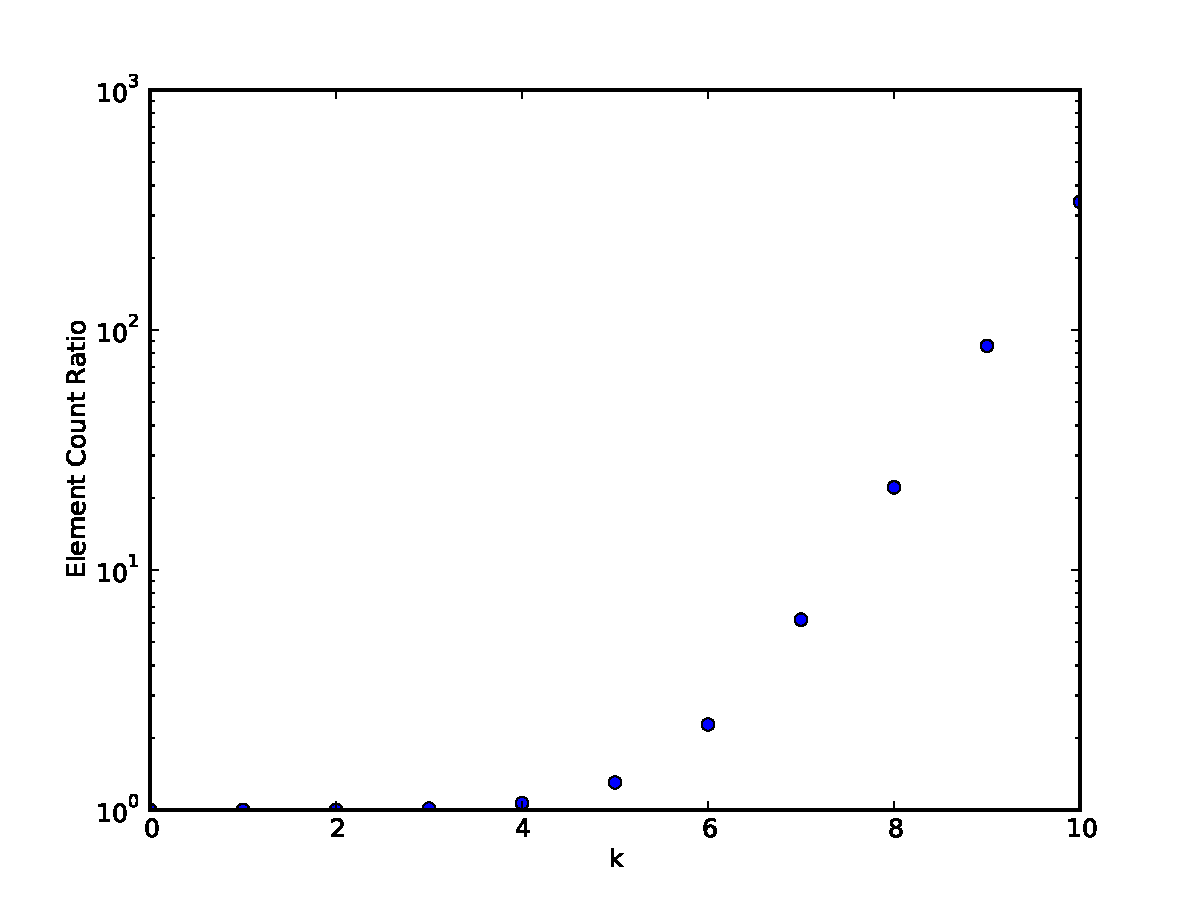
\includegraphics[width=0.8\textwidth]{Dissertation/Scaling/RatioElementCount.pdf}
\caption{Ratio of total element counts $E_{tot3}/E_{tot1}$}
\label{fig:ElementCountRatio}
\end{figure}

There are two possible reasons we might want to use approach 3 over approach 1.
The first is speed, if the sum of the solve times for each individual time slab is
less than the solve time for a single solve done with approach 1, this might be an
attractive option. In fact, for this test problem, we can directly compute this for
various numbers of time slabs. 
For the sake of comparison, the solve time is defined to be the total time to solve all
time slabs while adaptively refining to a resolution of $h=1/2^{10}$ 
with the default geometric multigrid settings in Camellia (discussed above).
We plot these results in Figure \ref{fig:TimeSlabSolveTime} and there does appear to be 
a sweet spot for this problem at 16 time slabs, but the potential speedup alone isn't 
enough to justify the more complicated implementation.
\begin{figure}
\centering
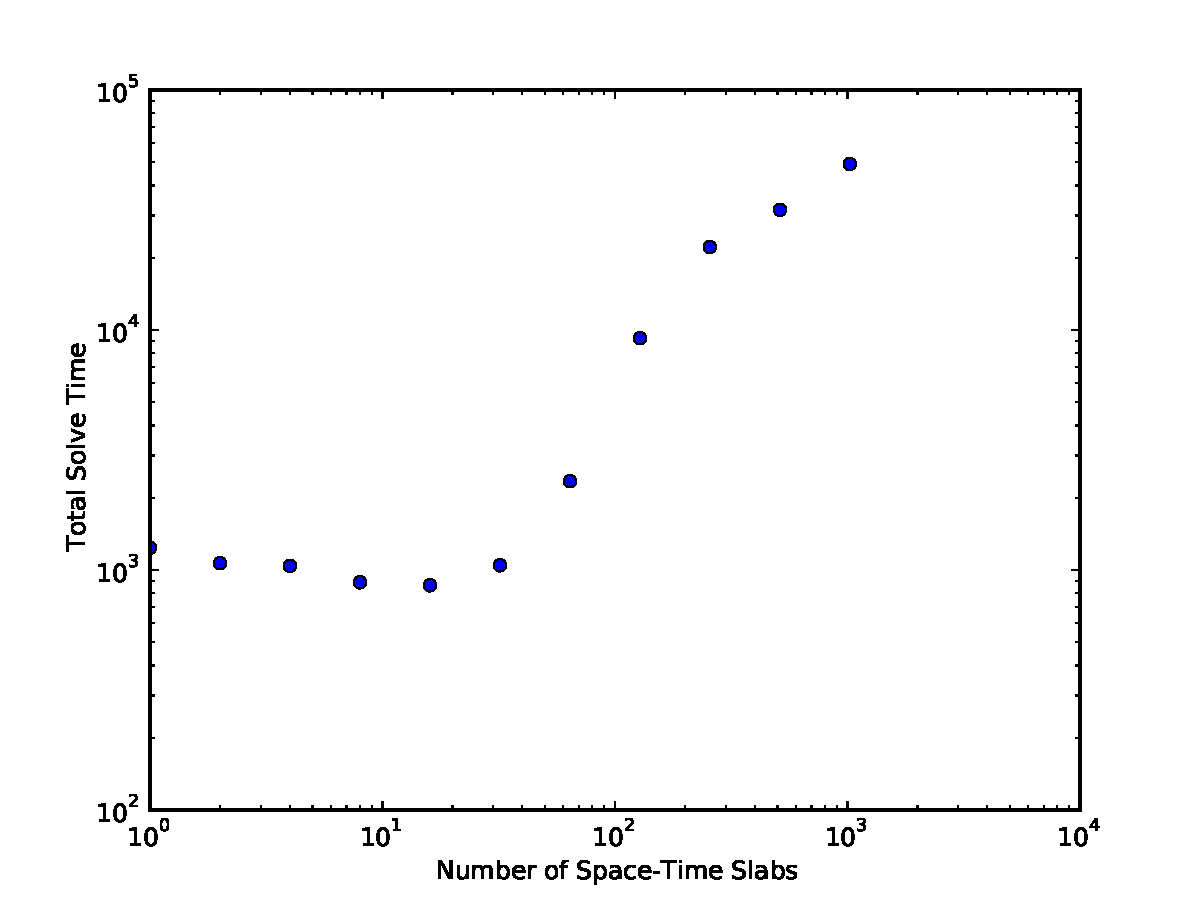
\includegraphics[width=0.8\textwidth]{Dissertation/Scaling/TimeSlabSolveTime.pdf}
\caption{Total solve time using strategy 3}
\label{fig:TimeSlabSolveTime}
\end{figure}

A more compelling reason has to do with memory. It is possible that for certain problems we might consider
the solution of the entire space-time domain might require more memory than is available.
By splitting the solve into smaller time slabs, you could mitigate produce smaller global solves that do 
fit into memory. So far, the memory constraint has not been a significant concern for the problems under
consideration here, so we opted to stick with the simplest approach, the first strategy.

\end{document}